\documentclass{article}
\usepackage{graphicx}

\begin{document}
any changes
\subsection{Power System (MKWJOH004)}
\label{sec:PowerSystem}
    \subsubsection{Context for design}
    The power system is required to power logic, sensing and stability system. Each of the system will have to be supplied with power based on the voltage and current ratings.
     \subsubsection{User Requirements}
\begin{tabular}{|c|p{7.2cm}|}
 \hline
 \textbf{SBRM1-0-001} &\textbf{DC power supply}  \\ 
 \hline
 \textbf{Requirement} & Most electronic circuits use DC power supply\\
 \hline
 \textbf{Rationale} & Motorbikes are powered by batteries which only store DC power and therefore the circuitry with will be powered by DC power supply. \\
 \hline
 \textbf{Refined By} & SBRM1-1-001, SBRM-2-001\\% other requirements that influence this one.
 \hline
 \textbf{Verification} & \\
 \hline
 \textbf{Relevance to system} & Will be used to power sensing and logic subsystems\\
 \hline
\end{tabular}\\[0.5cm]


\begin{figure}[ht]
        \centering
        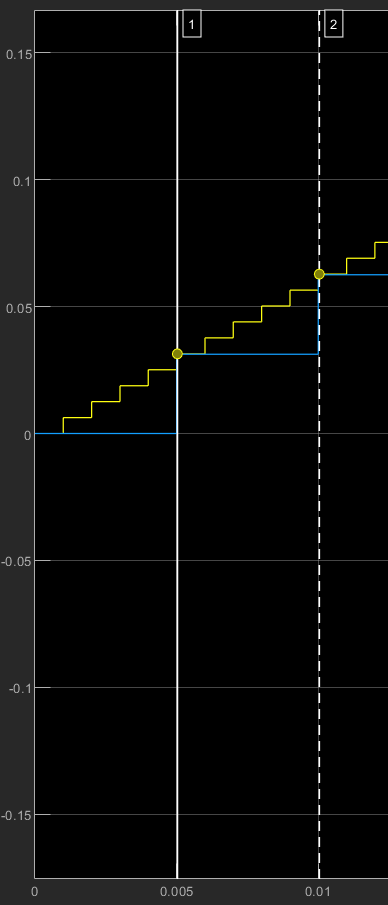
\includegraphics[height = 50mm]{pic/acc_zoom.PNG}
        \caption{Comparing True Value vs Sensor Output}
\end{figure}

\paragraph{}
why doesnt the git hub changes work

\end{document}